% ============================================================
% FORMULA 1 PIT STOP PREDICTION AND ANOMALY DETECTION
% Machine Learning Report
% ============================================================

\documentclass[11pt,a4paper]{report}

% ============================================================
% PACKAGES
% ============================================================

% Encoding and fonts
\usepackage[utf8]{inputenc}
\usepackage[T1]{fontenc}
\usepackage{lmodern}

% Math packages
\usepackage{amsmath}
\usepackage{amssymb}
\usepackage{amsfonts}

% Graphics and figures
\usepackage{graphicx}
\usepackage{float}
\usepackage{caption}

% TikZ for diagrams
\usepackage{tikz}
\usetikzlibrary{positioning, shapes.geometric, arrows.meta}

% Tables
\usepackage{booktabs}
\usepackage{multirow}

% Formatting
\usepackage[margin=2.5cm]{geometry}
\usepackage{setspace}
\usepackage{parskip}

% Hyperlinks and references
\usepackage{hyperref}
\hypersetup{
    colorlinks=true,
    linkcolor=blue,
    citecolor=blue,
    urlcolor=blue,
    pdftitle={F1 Pit Stop Prediction and Anomaly Detection},
    pdfauthor={Student Name}
}

% Code listings (if needed)
\usepackage{listings}
\usepackage{xcolor}

% Table of contents depth
\setcounter{tocdepth}{2}
\setcounter{secnumdepth}{2}

% ============================================================
% DOCUMENT BEGIN
% ============================================================

\begin{document}
\onehalfspacing

% ============================================================
% PART 0 — TITLE PAGE & ABSTRACT (SHORTENED)
% ============================================================

\begin{titlepage}
    \centering
    \vspace*{2cm}

    {\Huge \textbf{Predictive Pit Stop Strategy and Anomaly Detection in Formula 1}}\\[1.2cm]
    {\Large Machine Learning and Telemetry Analysis}\\[0.8cm]

    {\large \textbf{Timothée Mariotte \\ Matthieu Puiseux \\ Jhon Liu}}\\
    {\large ESILV — Academic Year 2025–2026}\\[2cm]

    \vfill
\end{titlepage}

\chapter*{Abstract}
\addcontentsline{toc}{chapter}{Abstract}

This project builds a system that predicts pit stop timing and detects abnormal laps in Formula 1 using FastF1 telemetry.  
A multi-head XGBoost model estimates pit windows, next-lap pit probability, and pit timing, while a set of anomaly models highlights unusual behaviour.  
A Streamlit dashboard visualises predictions and telemetry, making the system easy to understand and explore.

% (Aucune image dans cette partie dans la version longue)


% ============================================================
% PART 1 — INTRODUCTION (SHORTENED)
% ============================================================

\chapter{Introduction}

Pit stop timing strongly influences race outcomes in Formula 1. Tyre wear, pace evolution, and driver behaviour make prediction difficult.  
With publicly available FastF1 telemetry, it becomes possible to build simple machine learning models that estimate pit windows and detect abnormal laps.

The system developed here includes:
\begin{itemize}
    \item a pit stop prediction model,
    \item an anomaly detection module,
    \item a decision fusion mechanism,
    \item a Streamlit dashboard.
\end{itemize}

\section*{Challenges}

Main challenges include incomplete telemetry for older seasons, strong differences between tracks, unpredictable race events, and varying driving styles.

\section*{Model Version Note}

Early figures in this report were generated before several improvements, including a next-lap pit classifier and updated fusion logic, which increased pit timing accuracy.

\section*{Objectives}

The report explains:
\begin{itemize}
    \item data preparation,
    \item feature engineering,
    \item model training,
    \item anomaly detection,
    \item decision fusion,
    \item dashboard implementation.
\end{itemize}


% ============================================================
% PART 2 — BUSINESS CASE (SHORTENED)
% ============================================================

\chapter{Business Case}

Pit stop timing affects race strategy, pace, and tyre life. Predicting pit windows helps engineers evaluate when a stop becomes optimal.  
Anomaly detection adds awareness of mechanical or performance issues that could trigger early stops.

\section{Why It Matters}

A prediction system can:
\begin{itemize}
    \item offer a consistent data-based reference,
    \item support engineers under pressure,
    \item reveal unexpected pace changes,
    \item provide learning and analysis value.
\end{itemize}

\section{Anomaly Detection Role}

Anomalies may indicate overheating, braking issues, traction loss, or traffic disturbances.  
Detecting them helps differentiate normal degradation from unusual behaviour.

\section{Decision Fusion}

Strategy signals and anomaly severity are combined into simple messages:
\begin{itemize}
    \item Continue,
    \item Monitor,
    \item Pit Now.
\end{itemize}

\section{Dataset Limitations}

Telemetry gaps restrict modelling to seasons with complete data.

\section*{Summary}

The system provides:
\begin{enumerate}
    \item strategic signals,
    \item mechanical awareness,
    \item interpretable outputs,
    \item an educational tool.
\end{enumerate}

% (Aucune image dans la version longue pour cette partie)


% ============================================================
% PART 3 — DATASET DESCRIPTION (SHORTENED)
% ============================================================

\chapter{Dataset Description}

The project uses FastF1 telemetry and lap timing data from Formula 1 races.  
Only Race sessions are used, as they determine pit timing and performance variations.

\section{Types of Data}

FastF1 provides:
\begin{itemize}
    \item lap timing (lap time, sectors, tyre info, flags),
    \item telemetry (speed, throttle, brake, RPM, DRS),
    \item weather (temperatures, wind, rain),
    \item metadata (drivers, circuit info).
\end{itemize}

\section{Data Structure}

For each driver–race:
\begin{itemize}
    \item ~50–70 laps,
    \item ~20–40 engineered features per lap,
    \item aggregated telemetry metrics,
    \item stint-level and contextual variables.
\end{itemize}

\section{Dashboard Example}

\begin{figure}[H]
    \centering
    \includegraphics[width=\textwidth]{Max-Verstappen-MonacoGP-2018-view-dashboard.png}
    \caption{Dashboard example for Max Verstappen — Monaco GP 2018.}
\end{figure}

\section{Limitations}

Older seasons may lack key telemetry such as throttle, brake, or tyre age.  
Only complete seasons were used for modelling.

\section*{Summary}

FastF1 provides a detailed race dataset suitable for modelling, though uneven historical coverage limits available training samples.


% ============================================================
% PART 4 — PREPROCESSING & FEATURE ENGINEERING (SHORTENED)
% ============================================================

\chapter{Data Preprocessing and Feature Engineering}

Raw telemetry requires cleaning, alignment, and aggregation before modelling.

\section{Cleaning Steps}

\begin{itemize}
    \item removal of invalid laps,
    \item interpolation of telemetry gaps,
    \item standardisation of times and tyre fields,
    \item conversion of time formats.
\end{itemize}

\section{Lap-Level Aggregation}

Telemetry is summarised per lap:
\begin{itemize}
    \item mean/max/min speed,
    \item throttle ratio,
    \item brake percentage,
    \item DRS usage,
    \item RPM and acceleration metrics.
\end{itemize}

\begin{figure}[H]
    \centering
    \includegraphics[width=\textwidth]{Max-Verstappen-MonacoGP-2018-sensors-throttle-break-speed.png}
    \caption{Aggregated telemetry signals: throttle, brake, speed.}
\end{figure}

\section{Stint and Weather Features}

\begin{itemize}
    \item tyre age, laps since last stop,
    \item stint progress,
    \item track/air temperature, wind.
\end{itemize}

\section{Rolling Features}

\begin{itemize}
    \item rolling lap time mean,
    \item lap deltas,
    \item rolling speed variability.
\end{itemize}

\section*{Summary}

The final dataset combines telemetry, stint context, and temporal structure, enabling tyre and pace modelling.


% ============================================================
% PART 5 — STRATEGY MODEL (SHORTENED)
% ============================================================

\chapter{Predictive Strategy Model}

Pit timing is predicted using a \textbf{multi-head XGBoost model}.

\section{Why XGBoost}

\begin{itemize}
    \item strong performance on tabular data,
    \item handles non-linear interactions,
    \item interpretable feature importance,
    \item robust to noise.
\end{itemize}

\section{Model Outputs}

Three heads provide:
\begin{enumerate}
    \item pit window classification (imminent / soon / later),
    \item regression of laps until next pit,
    \item next-lap pit probability.
\end{enumerate}

\section{Insights and Evaluation}

\begin{figure}[H]
    \centering
    \includegraphics[width=\textwidth]{Max-Verstappen-MonacoGP-2018-strategy-model-insights.png}
    \caption{Pit window predictions — Monaco GP 2018.}
\end{figure}

\begin{figure}[H]
    \centering
    \includegraphics[width=0.9\textwidth]{Max-Verstappen-MonacoGP-2018-strategy-model-feature-importance-PitWindow.png}
    \caption{Feature importance for pit window prediction.}
\end{figure}

\begin{figure}[H]
    \centering
    \includegraphics[width=\textwidth]{Max-Verstappen-MonacoGP-2018-pitstop-graph-prediction.png}
    \caption{Pit urgency curve vs real pit stop — Monaco 2018.}
\end{figure}

\section{Additional Examples}

\begin{figure}[H]
    \centering
    \includegraphics[width=\textwidth]{Other-example-Lewis-Hamilton-CanadianGP-2022-pitstop-graph-prediction-2-stops.png}
    \caption{Two-stop prediction example — Hamilton, Canada 2022.}
\end{figure}

\begin{figure}[H]
    \centering
    \includegraphics[width=\textwidth]{Other-example-Pierre-Gasly-BahrainGP-2023-pitstop-graph-prediction-3-stops.png}
    \caption{Three-stop prediction example — Gasly, Bahrain 2023.}
\end{figure}

\section{Evaluation}

Metrics:
\begin{itemize}
    \item Macro-F1 for pit window,
    \item MAE for pit timing,
    \item calibration curves for next-lap prediction.
\end{itemize}

\section*{Summary}

The strategy model provides reliable pit window predictions and forms the basis of the decision fusion layer.

% ============================================================
% PART 6 — ANOMALY DETECTION MODELS (SIMPLIFIED)
% ============================================================

\chapter{Anomaly Detection Models}

Unexpected events such as mechanical issues, tyre overheating, or sudden pace drops  
can change pit stop timing. To capture these cases, the project includes an  
\textbf{anomaly detection module} based on telemetry and pace behaviour.

\section{Motivation for Telemetry-Based Anomaly Detection}

Typical anomalies include:

\begin{itemize}
    \item brake or tyre overheating,
    \item loss of grip or traction issues,
    \item engine irregularities,
    \item driver mistakes,
    \item slow laps caused by traffic or flags,
    \item inconsistent sensor data.
\end{itemize}

Detecting these events helps understand performance drops that may influence pit decisions.

\section{Feature Set for Anomaly Detection}

The anomaly models use features such as:

\begin{itemize}
    \item lap time,
    \item tyre life and stint number,
    \item mean/max/min speed,
    \item throttle and brake usage,
    \item DRS flag,
    \item rolling pace metrics,
    \item acceleration values,
    \item weather data.
\end{itemize}

Before training, the following laps are removed:

\begin{itemize}
    \item pit laps,
    \item laps extremely slower than normal,
    \item formation or restart laps.
\end{itemize}

\section{Autoencoder Model}

A shallow Autoencoder compresses each lap into a small latent space  
and reconstructs it. The anomaly score is the reconstruction error:

\[
\text{Error}(x) = \| x - \hat{x} \|_1.
\]

High error indicates unusual telemetry patterns.

\section{Isolation Forest}

Isolation Forest detects anomalies by isolating points that require  
fewer random splits. It works well with high-dimensional features  
and noisy data.

\section{One-Class SVM}

One-Class SVM defines the boundary of normal laps and flags points  
that fall outside this boundary. It is useful for detecting subtle deviations.

\section{Fusion of Anomaly Models}

To stabilize predictions, the three models are combined:

\[
\text{AnomalyScore} = 0.5\,\text{AE} + 0.3\,\text{IF} + 0.2\,\text{OCS}.
\]

Each race computes its own threshold (99.5th percentile):

\[
\text{IsAnomaly}(x) =
\begin{cases}
1, & \text{if score > threshold},\\
0, & \text{otherwise}.
\end{cases}
\]

This adapts the detection to circuit-specific pace variations.

\section{Examples of Detected Anomalies}

\begin{figure}[H]
    \centering
    \includegraphics[width=\textwidth]{Example-anomaly-lap-graph-Lewis-hamilton-2022-CanadianGP.png}
    \caption{Anomaly score for Hamilton, 2022 Canadian GP.}
\end{figure}

\begin{figure}[H]
    \centering
    \includegraphics[width=0.9\textwidth]{Example-anomaly-lap-Lewis-hamilton-2022-CanadianGP.png}
    \caption{Telemetry traces for anomalous laps.}
\end{figure}

Detected anomalies often correspond to braking issues, traction loss,  
pace drops, or traffic disturbances.

\section{Limitations}

\begin{itemize}
    \item yellow-flag slowdowns may be misclassified as anomalies,
    \item telemetry noise can produce false positives,
    \item quality depends on accurate filtering of “normal” laps,
    \item anomalies do not always require a pit stop.
\end{itemize}

\section*{Summary}

The anomaly detection module highlights laps with unusual behaviour  
that may affect strategy. By combining three models and adapting thresholds  
per race, the system provides a reliable complement to pit stop prediction.

% ============================================================
% PART 7 — DECISION FUSION (SIMPLIFIED)
% ============================================================

\chapter{Decision Fusion}

Pit stop timing depends on tyre wear, pace evolution, driver behaviour,  
environmental conditions, and unexpected issues.  
To combine all signals into one clear output, the project uses a  
\textbf{decision fusion layer} that merges strategy predictions with  
anomaly scores.

\section{Motivation for Multi-Signal Fusion}

Strategy predictions alone may miss sudden events such as:

\begin{itemize}
    \item sharp pace drops,
    \item mechanical issues,
    \item telemetry irregularities,
    \item environmental changes,
    \item traffic disturbances.
\end{itemize}

The anomaly module captures these behaviours, so both sources must be merged  
to give a usable race recommendation.

\section{Components of the Fusion System}

The fusion layer uses four signals:

\begin{enumerate}
    \item pit window probabilities,
    \item next-lap pit probability,
    \item PitUrgency score (combined strategy signals),
    \item anomaly severity.
\end{enumerate}

These are combined into a single \textbf{DecisionScore}.

\section{Fusion of Strategy Signals}

Strategy signals are merged as:

\[
\text{PitUrgency} =
0.5 P_{\text{NextLap}} +
0.7 P_{\text{Imminent}} +
0.3 P_{\text{Soon}}.
\]

This gives more weight to imminent pit windows and next-lap predictions.

\section{Fusion of Anomaly Signals}

The anomaly module outputs a normalized score:

\[
\text{AnomalySeverity} \in [0,1].
\]

High values indicate strong mechanical or performance risk.

\section{Final Decision Score}

The unified score is:

\[
\text{DecisionScore} = 100 \cdot
\left(0.6\,\text{PitUrgency} + 0.4\,\text{AnomalySeverity}\right).
\]

Strategy dominates (60%), but anomalies still have significant influence.

\section{Decision Messages}

The score is mapped to simple messages:

\begin{itemize}
    \item \textbf{Continue} — low urgency,
    \item \textbf{Monitor} — medium urgency or growing risk,
    \item \textbf{Pit Now} — high urgency.
\end{itemize}

If a strong anomaly is detected:

\[
\text{If IsAnomaly = 1} \rightarrow \text{``Alert: abnormal telemetry''}.
\]

\section{Interpretation and Practical Behaviour}

Observed behaviour across races:

\begin{itemize}
    \item PitUrgency rises steadily with tyre wear,
    \item anomaly spikes trigger warning messages,
    \item DecisionScore peaks near real pit stops,
    \item multi-stop races show multiple urgency cycles.
\end{itemize}

\section{Limitations}

\begin{itemize}
    \item safety car events cannot be predicted from telemetry,
    \item driver styles influence urgency curves,
    \item circuits differ in degradation characteristics,
    \item anomalies do not always mean a pit stop is needed.
\end{itemize}

\section*{Summary}

The fusion layer combines strategy predictions and anomaly signals  
into a single interpretable recommendation.  
It forms the main operational output of the full predictive system.


% ============================================================
% PART 8 — STREAMLIT DASHBOARD (SIMPLIFIED)
% ============================================================

\chapter{Interactive Dashboard (Streamlit UI)}

The machine learning models produce useful predictions, but users need  
a clear way to explore and interpret them.  
For this reason, the project includes an \textbf{interactive Streamlit dashboard}  
that displays telemetry, predictions, anomalies, and pit comparisons.

\section{Motivation for a Visual Interface}

A visual interface helps users:

\begin{itemize}
    \item understand why the model predicts a pit stop,
    \item relate anomalies to lap times and telemetry,
    \item compare predictions with real pit stops,
    \item observe degradation and pace trends.
\end{itemize}

Thus, the dashboard acts as both a presentation and diagnostic tool.

\section{Dashboard Structure}

The UI is organized into several components:

\begin{itemize}
    \item \textbf{Session Filters}: race year, event, driver, lap selection.
    \item \textbf{KPIs}: number of anomalies, average pit urgency, average decision score.
    \item \textbf{Anomaly Module}: list of anomalous laps, scores, and lap-time outliers.
    \item \textbf{Strategy Insights}: pit window predictions, next-lap probability, decision score.
    \item \textbf{Pit Stop Comparison}: predicted vs. real pit laps.
    \item \textbf{Telemetry Overview}: speed, throttle, brake, and other sensor summaries.
\end{itemize}

\section{Illustration of the Dashboard UI}

\begin{figure}[H]
    \centering
    \includegraphics[width=\textwidth]{Max-Verstappen-MonacoGP-2018-view-dashboard.png}
    \caption{Streamlit dashboard example for Monaco 2018.}
\end{figure}

The dashboard provides a simple, interactive way to explore all model outputs.

\section{Integration with the Predictive Pipeline}

The dashboard loads the processed dataset containing:

\begin{itemize}
    \item pit window predictions,
    \item next-lap recommendations,
    \item pit urgency and probabilities,
    \item anomaly flags and severity,
    \item final decision score and message.
\end{itemize}

Because Streamlit updates interactively, all charts refresh instantly  
when filters change.

\section{Role in Model Development}

During development, the dashboard was used to:

\begin{itemize}
    \item debug feature engineering,
    \item compare predictions with real pit stops,
    \item analyse anomalies alongside telemetry,
    \item present results clearly.
\end{itemize}

It also revealed behaviours such as:

\begin{itemize}
    \item degradation patterns aligned with anomaly spikes,
    \item anomalies caused by traffic rather than tyre issues,
    \item changes in pace during Safety Car phases.
\end{itemize}

\section{Benefits of a Visual Analytics Layer}

The dashboard improves:

\begin{itemize}
    \item \textbf{interpretability} — why predictions occur,
    \item \textbf{explainability} — links between features and outputs,
    \item \textbf{context awareness} — predictions within the race timeline,
    \item \textbf{user engagement} — interactive exploration.
\end{itemize}

\section*{Summary}

The Streamlit dashboard is the main interface for examining predictions,  
anomalies, and telemetry behaviour.  
It plays a key role in model evaluation and makes the system practical  
for real analysis.

% ============================================================
% PART 9 — LIMITATIONS (SHORTENED)
% ============================================================

\chapter{Limitations}

Although the system provides useful insights, several limits reduce its accuracy and reliability.

\section{Race Incidents Cannot Be Predicted}

The model cannot anticipate events such as:

\begin{itemize}
    \item Safety Cars or Virtual Safety Cars,
    \item crashes and debris,
    \item sudden weather changes,
    \item red-flag interruptions.
\end{itemize}

These events are external to telemetry and disrupt normal race patterns.  
During SC/VSC conditions:

\begin{itemize}
    \item lap times drop sharply,
    \item degradation slows,
    \item pit-loss time decreases,
    \item strategy depends on context, not telemetry.
\end{itemize}

Thus, pit decisions under SC/VSC must remain manual.

\section{Data Limitations}

\subsection*{Incomplete Historical Telemetry}

Older seasons (e.g., 2018–2019) contain:

\begin{itemize}
    \item missing throttle/brake/RPM data,
    \item irregular sampling,
    \item incomplete tyre metadata.
\end{itemize}

This restricts the usable dataset and reduces training diversity.

\subsection*{Telemetry Noise}

Telemetry may include:

\begin{itemize}
    \item sampling noise,
    \item desync between channels,
    \item missing packets.
\end{itemize}

Even after cleaning, residual noise affects predictions and anomaly scores.

\section{Model Limitations}

\subsection*{Approximate Representation of Tyre Behaviour}

XGBoost uses correlations, but true tyre behaviour depends on factors not in the data  
(temperature cycles, surface grip, sliding, asphalt properties).  
The model remains an approximation.

\subsection*{Driver Behaviour Variability}

Drivers differ in braking style, tyre management, and pace control.  
This reduces generalisation across drivers.

\subsection*{Circuit Variability}

Tracks differ in degradation, layout, asphalt, and pit-loss time.  
This makes universal modelling difficult with limited data.

\section{Anomaly Detection Limits}

Anomalies detected by the model may represent:

\begin{itemize}
    \item driver mistakes,
    \item temporary overheating,
    \item traffic effects,
    \item yellow flags,
    \item aggressive tyre saving,
    \item sensor noise.
\end{itemize}

Many do not imply the need for a pit stop.  
Thus, anomaly detection is informative but not prescriptive.

\section{Operational Constraints}

Real-time deployment in F1 would require:

\begin{itemize}
    \item high-frequency telemetry streaming,
    \item very low latency,
    \item integration with simulation tools,
    \item expert supervision.
\end{itemize}

So, in this configuration, and for the moment, the system is designed for analysis, not live race control.

\section{Human Expertise Still Required}

Engineers must interpret:

\begin{itemize}
    \item traffic and overtaking chances,
    \item undercut/overcut potential,
    \item weather forecasts,
    \item competitor strategy,
    \item tyre allocation limits.
\end{itemize}

The model provides support, not automated decision-making.

\section*{Summary}

The framework offers useful insights into pit timing and anomalies,  
but unpredictable race events, incomplete telemetry, driver and circuit differences,  
and operational constraints limit predictive accuracy.  
Despite this, it provides a solid basis for future improvements.

% ============================================================
% PART 10 — CONCLUSION (SHORTENED)
% ============================================================

\chapter{Conclusion}

This project developed a complete data-driven framework to analyse Formula 1 telemetry,  
predict pit stop timing, detect anomalies, and combine these signals into a simple  
decision-support tool. Using open-source data and accessible ML methods, the system shows  
that key aspects of race strategy can be approximated in an interpretable way.

\section*{Summary of Contributions}

Main achievements include:

\begin{itemize}
    \item a preprocessing pipeline that converts raw telemetry into usable features,
    \item a multi-head XGBoost model predicting pit windows and next-lap pit probability,
    \item an anomaly detection module combining three complementary algorithms,
    \item a decision fusion layer producing clear messages (“Continue”, “Monitor”, “Pit Now”),
    \item an interactive Streamlit dashboard for exploring predictions and telemetry.
\end{itemize}

Together, these components form a consistent analytical system for studying tyre wear,  
pace evolution, and strategy signals.

\section*{Interpretation and Relevance}

The framework does not replace professional race simulators but shows that machine learning  
can capture useful patterns from public telemetry. It helps:

\begin{itemize}
    \item identify degradation trends,
    \item anticipate pit windows in normal race conditions,
    \item flag abnormal laps,
    \item visualise race dynamics clearly.
\end{itemize}

This makes it a practical educational tool for understanding F1 strategy.

\section*{Limitations and Challenges}

The system is limited by incomplete telemetry, driver variability, noise in raw signals,  
and the impossibility of predicting race incidents such as Safety Cars.  
Human oversight remains essential for real strategy decisions.

\section*{Future Work}

Potential extensions include:

\begin{itemize}
    \item real-time inference with live telemetry,
    \item adding weather and track evolution models,
    \item tyre wear simulation to complement ML predictions,
    \item driver-specific calibration,
    \item comparative multi-driver analysis.
\end{itemize}

These additions would move the system closer to operational use.

\section*{Closing Remarks}

The project shows that telemetry, machine learning, anomaly detection, and visualisation  
can be combined to create an accessible analysis platform for Formula 1 racing.  
While simplified compared to professional systems, it provides a solid foundation  
for future exploration and highlights how data-driven tools can support human expertise  
in one of the most complex and dynamic sports.

% ============================================================
% PART 11 — GLOSSARY (UNCHANGED)
% ============================================================

\chapter*{Glossary}
\addcontentsline{toc}{chapter}{Glossary}

\begin{description}
    \item[Anomaly Detection] ML techniques used to identify laps with unusual telemetry.
    \item[Autoencoder] A neural network that compresses and reconstructs inputs; high error suggests abnormality.
    \item[Brake Percentage] Fraction of a lap where braking is applied.
    \item[Decision Fusion] Method combining strategy and anomaly signals into a final recommendation.
    \item[DRS] Drag Reduction System used to reduce drag on straights.
    \item[Feature Engineering] Transforming raw telemetry into model-ready variables.
    \item[Isolation Forest] Anomaly detector using random partitioning.
    \item[Lap Delta] Difference between two consecutive lap times.
    \item[Next-Lap Pit Probability] Probability that a driver will pit on the next lap.
    \item[One-Class SVM] Model that defines the boundary of normal telemetry.
    \item[Pit Stop] Entering the pit lane to change tyres or repair the car.
    \item[Pit Window] The race interval where a pit stop becomes optimal.
    \item[PitUrgency] Score summarising pit timing likelihood.
    \item[Reconstruction Error] Autoencoder-based anomaly metric.
    \item[Rolling Feature] Metric computed across several laps to capture trends.
    \item[Safety Car] Race neutralisation that drastically slows the field.
    \item[Stint] Sequence of laps on one tyre set.
    \item[Streamlit] Library for building interactive dashboards.
    \item[Telemetry] High-frequency car sensor data.
    \item[XGBoost] Gradient boosting algorithm for predictive modelling.
\end{description}

% ============================================================
% PART 12 — APPENDICES (SHORTENED)
% ============================================================

\appendix

\chapter{Appendix A: Feature Table}

\begin{table}[H]
\centering
\begin{tabular}{|l|p{8cm}|}
\hline
\textbf{Feature} & \textbf{Description} \\ \hline
LapTime & Lap time in seconds. \\ \hline
TyreLife & Tyre age in laps. \\ \hline
MeanSpeed & Average lap speed. \\ \hline
ThrottleRatio & Full-throttle percentage. \\ \hline
BrakeRatio & Braking percentage. \\ \hline
RollingLapMean & Rolling mean lap time. \\ \hline
PaceDrift & Short vs. long pace difference. \\ \hline
StintLength & Laps in current stint. \\ \hline
TrackTemp & Track temperature. \\ \hline
DRSCount & Number of DRS activations. \\ \hline
\end{tabular}
\caption{Main engineered features used for modelling.}
\end{table}

\chapter{Appendix B: Python File Overview}

\begin{itemize}
    \item \texttt{data\_loader.py}: loading and filtering sessions.
    \item \texttt{feature\_engineering.py}: rolling features and telemetry summaries.
    \item \texttt{strategy\_model.py}: XGBoost pit prediction.
    \item \texttt{anomaly\_model.py}: Autoencoder + Isolation Forest + One-Class SVM.
    \item \texttt{decision\_fusion.py}: merging strategy and anomaly outputs.
    \item \texttt{dashboard.py}: Streamlit visual interface.
\end{itemize}

\chapter{Appendix C: Methodological Notes}

\begin{itemize}
    \item telemetry gaps handled via interpolation,
    \item stint detection based on tyre compound changes,
    \item Safety Car phases excluded from modelling.
\end{itemize}

% ============================================================
% PART 13 — PIPELINE TIKZ DIAGRAM
% ============================================================

\chapter{Pipeline Diagram}

\begin{figure}[H]
\centering
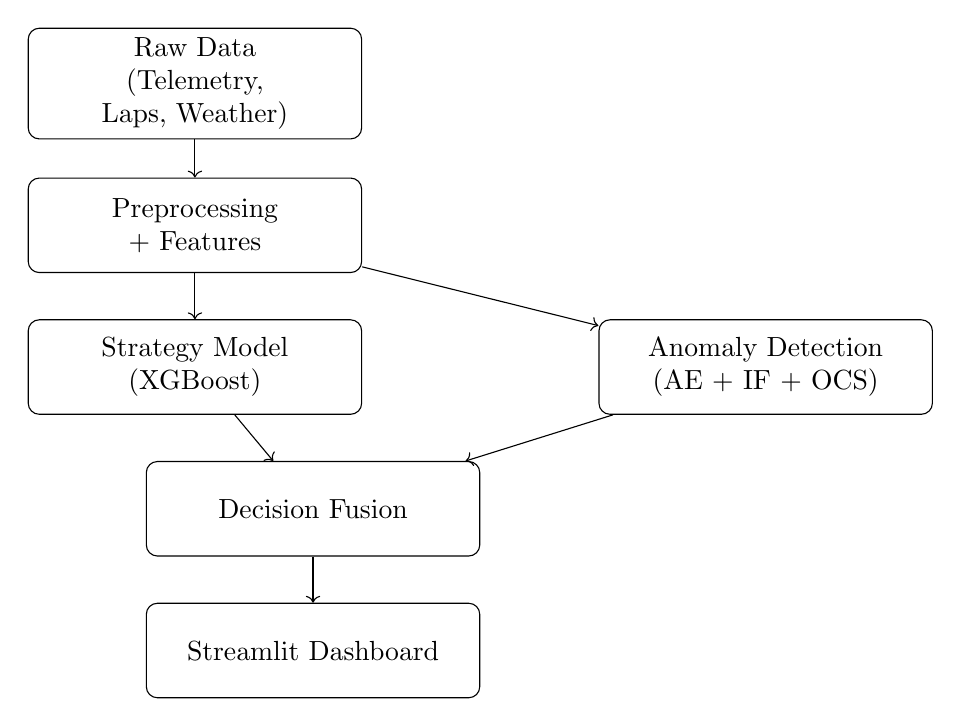
\begin{tikzpicture}[node distance=1.8cm, auto]

\tikzstyle{block} = [
    rectangle,
    draw,
    rounded corners,
    text width=4cm,
    align=center,
    minimum height=1.2cm
];

\node[block] (data) {Raw Data \\ (Telemetry, Laps, Weather)};
\node[block, below of=data] (prep) {Preprocessing \\ + Features};
\node[block, below of=prep] (strategy) {Strategy Model \\ (XGBoost)};
\node[block, right=3cm of strategy] (anomaly) {Anomaly Detection \\ (AE + IF + OCS)};
\node[block, below of=strategy, xshift=1.5cm] (fusion) {Decision Fusion};
\node[block, below of=fusion] (dashboard) {Streamlit Dashboard};

\draw[->] (data) -- (prep);
\draw[->] (prep) -- (strategy);
\draw[->] (prep) -- (anomaly);
\draw[->] (strategy) -- (fusion);
\draw[->] (anomaly) -- (fusion);
\draw[->] (fusion) -- (dashboard);

\end{tikzpicture}
\caption{Pipeline from raw telemetry to decision output.}
\end{figure}

% ============================================================
% END OF DOCUMENT
% ============================================================

\end{document}
